% CREATED BY DAVID FRISK, 2016
\chapter{Theory}
\label{chap:theory}

This section provides the theoretical background necessary to understand the research presented in this thesis. It covers the fundamental concepts of information theory, compression theory, and neural compression, as well as the specific architectures used as baselines in this work. The goal is to establish a solid theoretical foundation for the subsequent empirical evaluations and proposed improvements.

% 2.3 Compression Theory and Traditional Methods - DONE (TIM) - DONE (EMRIK)
\section{Compression Theory and Traditional Methods}

\textbf{Information Theory} Because information theory provides the basis for compression methods, its core concepts are introduced here before discussing compression itself. Entropy is key to information theory. It measures the uncertainty of a random variable and is computed from its probability distribution. More specifically, the uncertainty in a probability distribution is the expected negative log-probability of its outcomes. The entropy of a discrete distribution $p = {(p_i)}_i$ is defined as \[H(p) = -\sum_i p_i \log p_i,\] where the base of the logarithm determines the unit~\cite{Shannon1948}.

To illustrate with a weather example, suppose the true probabilities of ``rain'' and ``shine'' are $p_1 = 0.3$ and $p_2 = 0.7$, respectively. Then (using base-2 logs), \[H(p) = -(p_1 \log p_1 + p_2 \log p_2) \approx 0.61.\] Suppose the measurements are instead from Abu Dhabi, where the probabilities might be $p_1 = 0.01$ and $p_2 = 0.99$. The entropy is now approximately $0.06$. There is thus much less uncertainty about any given day compared to a place where it rains 30\% of the time. In this way, information entropy quantifies the inherent uncertainty in a distribution of events.

Entropy is central to compression because it indicates how compressible data is. High-entropy data is less predictable and therefore harder to compress, while low-entropy data has redundant patterns and is therefore easier to compress~\cite{Shannon1948}.

The other important information theory concept to understand in the context of compression is mutual information. Mutual information, formally defined as $I(X;Y)$ answers the question ``How much does one variable tell me about another?''~\cite{Shannon1948}.

\textbf{Compression} Compression, as originated in information theory by Shannon~\cite{Shannon1948}, is the process of encoding information using fewer bits than the original representation. Compression techniques can be broadly categorized into lossless and lossy methods. Lossless compression is based on two principles: distribution modeling, sometimes called entropy modeling, and entropy coding. Entropy modeling involves creating a probabilistic representation of the data, while entropy coding assigns shorter codes to more frequent symbols based on their probabilities, thereby minimizing the average code length. Entropy serves as the lower bound (in bits per symbol) for any lossless compression scheme. Lossy compression on the other hand allows for some loss of information in exchange for a higher rate of compression. This is typically achieved through techniques such as transform coding and quantization~\cite{Sayood2017}. The compression ratio (CR) is key to lossy compression methods, and is defined as the size of uncompressed data divided by the size of compressed data~\cite{Thomasian2022}. For the purpose of this thesis, the focus will be on lossy compression as this is more suitable for common downstream ML tasks where some loss of fidelity is acceptable as long as the relevant information for the task is preserved.

\textbf{Rate-Distortion Theory} Rate-distortion theory provides the fundamental framework for lossy compression, quantifying the minimum bitrate $R(D)$ required to represent data with acceptable distortion at most $D$. Building on entropy and mutual information introduced earlier, it formalizes the fundamental tradeoff between rate and fidelity central to lossy compression. The rate-distortion function is formally defined as \[R(D) = \min_{p(\hat{X}|X):\ E[d(X,\hat{X})] \leq D} I(X;\hat{X}),\] where $d(x,\hat{x})$ is a distortion measure, e.g., squared error, $E[\cdot]$ is the average over all data points or expectation, and the minimum bitrate is computed over all distributions $p(\hat{X}|X)$ achieving average distortion at most $D$. Shannon's rate-distortion theorem proves this isn't just a theoretical lower bound and practical codes exist that get arbitrarily close to $R(D)$ bits/symbols while keeping distortion below $D$.~\cite{Shannon1949}.

Distortion measures quantify the cost of representation between original data $X$ and its compressed reconstruction $\hat{X}$. They are essential in rate-distortion theory, where the goal is to minimize bitrate subject to $E[d(X,\hat{X})] \leq D$ for a chosen distortion threshold $D$. Widely used examples for distortion measures include the squared error (MSE) or the Hamming distance. MSE is defined as $d(x,\hat{x}) = {(x - \hat{x})}^2$, and is often used for numerical/time-series data due to its mathematical tractability. The Hamming distance on the other hand is defined as $d(x,\hat{x}) = \sum_i \mathbf{1}\{x_i \neq \hat{x}_i\}$, and is used for binary or categorical data~\cite[pp.~304--305]{Cover2006}.

In the ML context, particularly in automotive systems, or in fact IoT systems in general, rate-distortion analysis denotes the trade-off between efficiently handling large quantities of data and maximizing model performance. So in this sense, rate-distortion theory gives the theoretical framework to the downstream ML task challenges described in Section~\ref{sec:downstream-ml-and-dq}. Traditional lossy compression techniques can reduce data volume, but often at the cost of losing critical information necessary for accurate ML tasks such as predictive maintenance, anomaly detection, and fleet analytics~\cite{Marchioni2024}. The impact of this trade-off is well-documented in the literature. Cuza et al.~\cite{Cuza2024} for example, study the impact of lossy compression techniques on time series forecasting tasks and observe a constant trade-off between CR and forecasting accuracy. It is important to note, that, while the authors of this paper see impact of CR on task performance, it is not necessarily a negative impact and is dependent on various factors~\cite[pp.~654--655]{Cuza2024}.

\textbf{Traditional Compression Methods} Traditional compression methods, based on information theory principles, often fall short in automotive applications, especially as a precursor for downstream ML tasks. For video/image compression, traditional methods like JPEG are optimized for human perception (e.g., visual quality) rather than ML tasks or efficient downstream data use~\cite[p.~12]{Ma2020}. For time series data, algorithmic approaches like CHIMP or Gorilla depend on manually chosen parameters like window size and are sensitive to data characteristics such as entropy and signal variability. This limits their effectiveness in capturing the nuances required for accurate ML model performance in automotive contexts~\cite[pp.~37--38 and 47]{Johnsson2025}. These algorithmic approaches were investigated by Johnsson~\cite{Johnsson2025} in a previous Master's thesis project. This work builds upon this thesis by exploring neural alternatives for vehicle telemetry compression. These neural alternatives are more flexible and can be optimized for specific downstream tasks and data characteristics, potentially offering better performance in terms of the rate-distortion trade-off for ML tasks. As previously shown by Tirupathi et al.~\cite{Tirupathi2022}, model aware compression techniques have the potential to retain more task relevant information compared to traditional methods, which is key for achieving better performance for downstream ML tasks while still maintaining significant CR. 

% 2.4 Neural Compression - TBD (TIM) - DONE (EMRIK)
\section{Neural Compression}

In the most basic sense, neural, or sometimes learned compression, is the application of neural networks and related ML techniques to the task of data compression~\cite{Yang2022}. Neural compression has been shown to be an effective strategy for handling the data rate-utility trade-off in various domains. Studies as early as 2019 have shown that neural compression methods can outperform traditional compression techniques for image and video data, especially at low bitrates~\cite{Löhdefink2019}. The same has been shown for time series data~\cite{Zheng2023, Liu2024}. This approach has also been shown to be effective in resource-constrained environments, such as IoT systems, where the ability to retain task-relevant information while reducing data volume is crucial~\cite{Azar2022, Hodo2025}.

In the following sections, the basics of neural compression theory and the connection to relevant information theory concepts are outlined.

\textbf{Information Bottleneck Theory} While the theory presented by Shannon~\cite{Shannon1948} gives a theoretical framework for understanding the limits of compression, it falls short when it comes to learned compression as it only considers the maximum CR for a given distortion level, without considering the specific characteristics of the data or the downstream tasks. This shortcoming is addressed in the information bottleneck theory, which presents a more nuanced approach to the issue of compression. In order to maintain relevance for downstream tasks, we need to preserve as much relevant information as possible about the target label, not about the input data. This is the core idea of the information bottleneck theory, which formalizes the trade-off between compression and relevance as: \[\min_{p(\hat{X}|X)} I(X;\hat{X}) - \beta I(Y;\hat{X}),\] where $I(X;\hat{X})$ is the mutual information between the input data $X$ and its compressed representation $\hat{X}$, $I(Y;\hat{X})$ is the mutual information between the target label $Y$ and the compressed representation $\hat{X}$, and $\beta$ is a Lagrange multiplier that controls the trade-off between compression and relevance~\cite{Tishby2000}. 

Early work on attempting to understand the learning dynamics of deep neural networks (DNNs) have applied the information bottleneck theory in an attempt to explain how DNNs learn compressed representations of data while preserving relevant information for specific tasks~\cite[pp.~1-5]{Tishby2015}. The core of this idea is that the goal of any supervised learning algorithm is to capture a minimally sufficient statistic in the input required to express the output. This mirrors the goal of information bottleneck compression which claims that there exists a maximally compressed representation of the input which retains the maximum amount of information about the target label. Other works such as~\cite{Shwartz2017} have attempted to show that DNNs both fit the input in order to increase the mutual information between the target and the latent representation $I(T;Y)$ while also compressing the input by lowering the mutual information between the input and the latent representation $I(X;T)$. This work has however been criticized for its methodology and computation of mutual information. Much of the issue comes down to the fact that the layers of a DNN may appear to lower mutual information in certain cases, for example when using a tahn activation function, but this has been shown to be a measurement artifact and not true information bottleneck compression. Instead, DNNs just learn to map the input to consistent output values, effectively decorrelating the data structure. This process will be referred to as geometric compression. In order for a network to be able to discard information and thereby compress the input in an information bottleneck sense, additional measures, like explicit stochasticity or quantization, are required~\cite{Saxe2018, Goldfeld2020}. So how DNNs learn is debated. But it becomes clear that geometric compression, while being dependent on the architecture or the used activation functions, is key to how DNNs function. Modern neural compression research therefore almost always combines geometric compression with some form of information-theoretic compression.

\textbf{Autoencoders \& Vector Quantization} 
The implementation of lossy neural compression methods is firmly based on autoencoders (AEs) and more specifically on Rate-Distortion Variational Autoencoders (R-D VAEs)~\cite[pp.~145--146]{Yang2022}. Generally AEs are defined as DNNs that try to reconstruct their input. This implies that the target output is the input. For this, AEs are composed of an encoder, which produces a hidden or latent representation, and a decoder, which takes this representation as an input and tries to reconstruct the original input. AEs are trained end-to-end, which means that the encoder and the decoder are trained in tandem. The training goal is to make the latent representation take on meaningful properties~\cite{Chen2023}.

The main difference between AEs and VAEs, introduced by Kingma and Welling~\cite{Kingma2013}, is that VAEs pick from a distribution of points when assigning latent representations, while AEs are deterministic in nature~\cite{Chen2023}. Importantly, many modern learned compression methods are formulated in a VAE-style rate-distortion framework. This is because an AE is essentially a VAE with a degenerate (Delta) variational posterior distribution. A deterministic AE maps $x$ to a single point $\hat{z} = f(x)$; the variational posterior $q(z|x)$ then becomes a Delta distribution and therefore deterministic~\cite[pp.~145--146]{Yang2022}. The choice between using a stochastic encoder or a deterministic encoder with quantization is an ongoing debate in the research community. Because of the non-differentiability of quantization, and the resulting problems in end-to-end training of lossy compression models, there has been experimentation with stochastic encoders. Theis and Agustsson~\cite{Theis2021} summarize the advantages of stochastic encoders, and while there certainly are advantages to stochastic encoders, deterministic encoders are favored by most modern neural compression methods~\cite{Yang2022, Theis2021}. No matter which of these approaches are implemented, they both display the compromise between geometric compression and information-theoretic compression outlined above. In the case of deterministic encoders, which are the focus of this thesis, the information-theoretic compression is achieved via quantization, which will be introduced in more detail in the next paragraph.

Quantization is often used in neural compression to introduce true information-theoretic compression when using deterministic encoders. While there have been various approaches to achieving true compression of information in the context of information bottleneck using neural networks, such as the variational information bottleneck architecture~\cite{Alemi2016}, the approach that is presented in this thesis extends the traditional AE architecture with a VQ bottleneck in order to minimize the entropy. This idea is conceptually more similar to methods such as those presented in~\cite[pp.~1611--1630]{Strouse2016}. The VQ layer acts as a deterministic information bottleneck partitioning the input space $X$ into regions that map to the same discrete code $t$, discarding intra-cluster variations. By binning the continuous signal to a finite set of codes, the entropy of the signal is bounded by the number of bins. As mentioned in~\cite{Saxe2018}, the encoder cannot exhibit decreasing $I(X;T)$ without noise or stochasticity since the entropy is constant $H(T\mid X)$. It can however create sharper decision boundaries which allow the VQ bottleneck to more effectively quantize the input while discarding the more uninformative information. 

In neural compression methods, AE architectures are typically chosen based on the structure of the input signals, the computational restraints, and the target rate-distortion objective. For telemetry and other mutlimodal time series data convolutional neural networks (CNNs) and recurrent neural networks (RNNs) are popular design choices~\cite[pp.146--148]{Yang2022}. CNNs naturally excel at capturing local temporal patterns efficiently, while RNNs are used to model longer-range dependencies~\cite[pp.146--148]{Yang2022}. Both CNNs and RNNs are especially suitable for neural compression, because they use a more compact parametric representation than for example fully connected neural networks~\cite{Du2019}. Naturally, a lot of hybrid systems trying to combine CNNs and RNNs have also emerged over the years. In practice, this architectural choice is not only a modeling decision but also a systems decision. Lightweight designs usually avoid costly recurrent designs and prefer convolutional approaches when compression is deployed on resource-constrained edge devices with strict latency and memory budgets~\cite{Hodo2025, Johnston2019}. 

\section{Baseline Implementations}

In this section, the architectures of the established compression methods which are used as baselines are introduced in detail. If not stated otherwise in this section, all configurations for the models are identical to those of the respective authors. A detailed description of the training configurations used for the experiments is provided in the next chapter.

\subsection{Baseline 1: TCN-RNN}

The continuous-latent AE approach introduced by Zheng and Zhang~\cite{Zheng2023} serves as the basis for the continuous-latent baseline model. Their work includes two models, the TCN-RNN model and the TCN-ARNN model, as well as a model selection mechanism. For simplicity, the focus here is on the TCN-RNN model. The TCN-RNN model is representative of state-of-the-art continuous-latent neural time-series compression methods. Compared to vanilla AEs, its architecture is explicitly designed to capture long temporal dependencies and has demonstrated stronger rate-distortion performance. This makes it a suitable baseline for evaluating the proposed implementation against a competitive neural compressor. While the TCN-RNN architecture represents a state-of-the-art continuous-latent neural time-series approach, it is mainly included and highlighted in this work to show the limitations of neural compression methods which use continuous latents. Another point to note about the TCN-RNN model is its costly architectural design, namely deep temporal convolutional stacks with large receptive fields, recurrent (often sequential) decoding, and dense continuous latent representations. These components typically lead to increased FLOPs, higher activation memory, and longer inference latency.
% should we discuss the computational efficiency since we don't actually compare it anywhere?

The TCN-RNN model is composed of four main components: the TCN-RNN encoder, a linear projection that serves as the bottleneck, the GRU decoder, and a second linear projection. A complete overview of the TCN-RNN architecture is shown in Figure~\ref{fig:tcn-rnn-architecture}.

\begin{figure}[h]
\centering
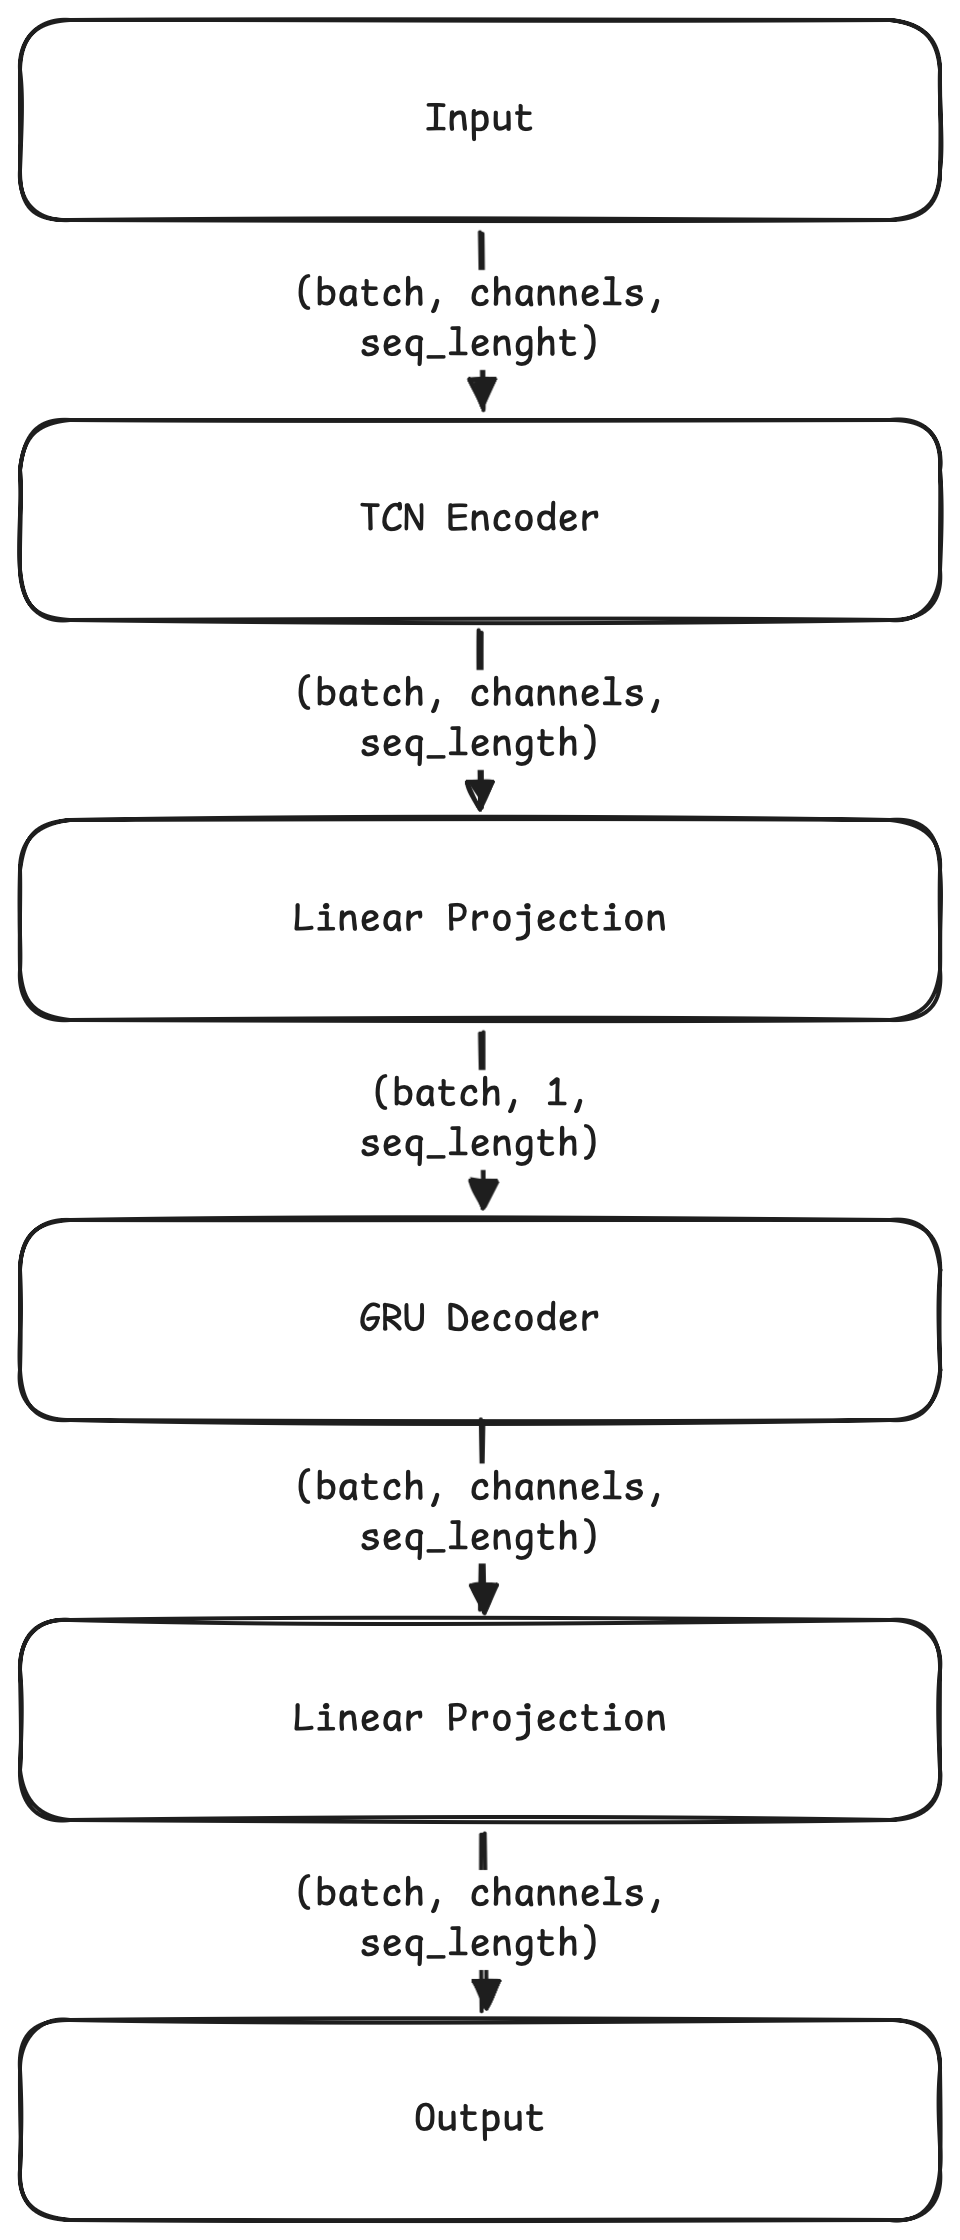
\includegraphics[width=0.40\linewidth]{figure/tcn-rnn.png}
\caption{TCN-RNN architecture} % Figure text below figure
\label{fig:tcn-rnn-architecture}
\end{figure}

The TCN encoder consists of a stack of temporal convolutional network (TCN) residual blocks with increasing dilation factors. Each TCN block is primarily composed of two causal convolutional layers, with normalization, a nonlinear activation function (ReLU), and optional dropout for regularization. Additionally, each TCN residual block implements a residual connection to stabilize training. The output is a continuous latent representation whose size is controlled by the downsampling factor and channel width. As in Zheng and Zhang~\cite{Zheng2023}, there is no downsampling in the decoder; any downsampling occurs in the linear bottleneck, which is described in the next paragraph. As a result, the input shape of the encoder is equal to its output shape. The detailed TCN encoder architecture is shown in Figure~\ref{fig:tcn-encoder}. In addition to common design choices such as dropout, residual connections, and the use of ReLU non-linearity, this encoder includes several noteworthy elements. It is designed with training efficiency and information preservation in mind. To this end, the authors use exponential dilations and additional layers to achieve stronger long-range temporal modeling. This design intentionally trades some computational efficiency for modeling capacity. The authors also employ weight normalization to improve training stability, which further increases computational cost.

\begin{figure}[h]
\centering
\subfloat[TCN encoder\label{fig:tcn-encoder}]{%
    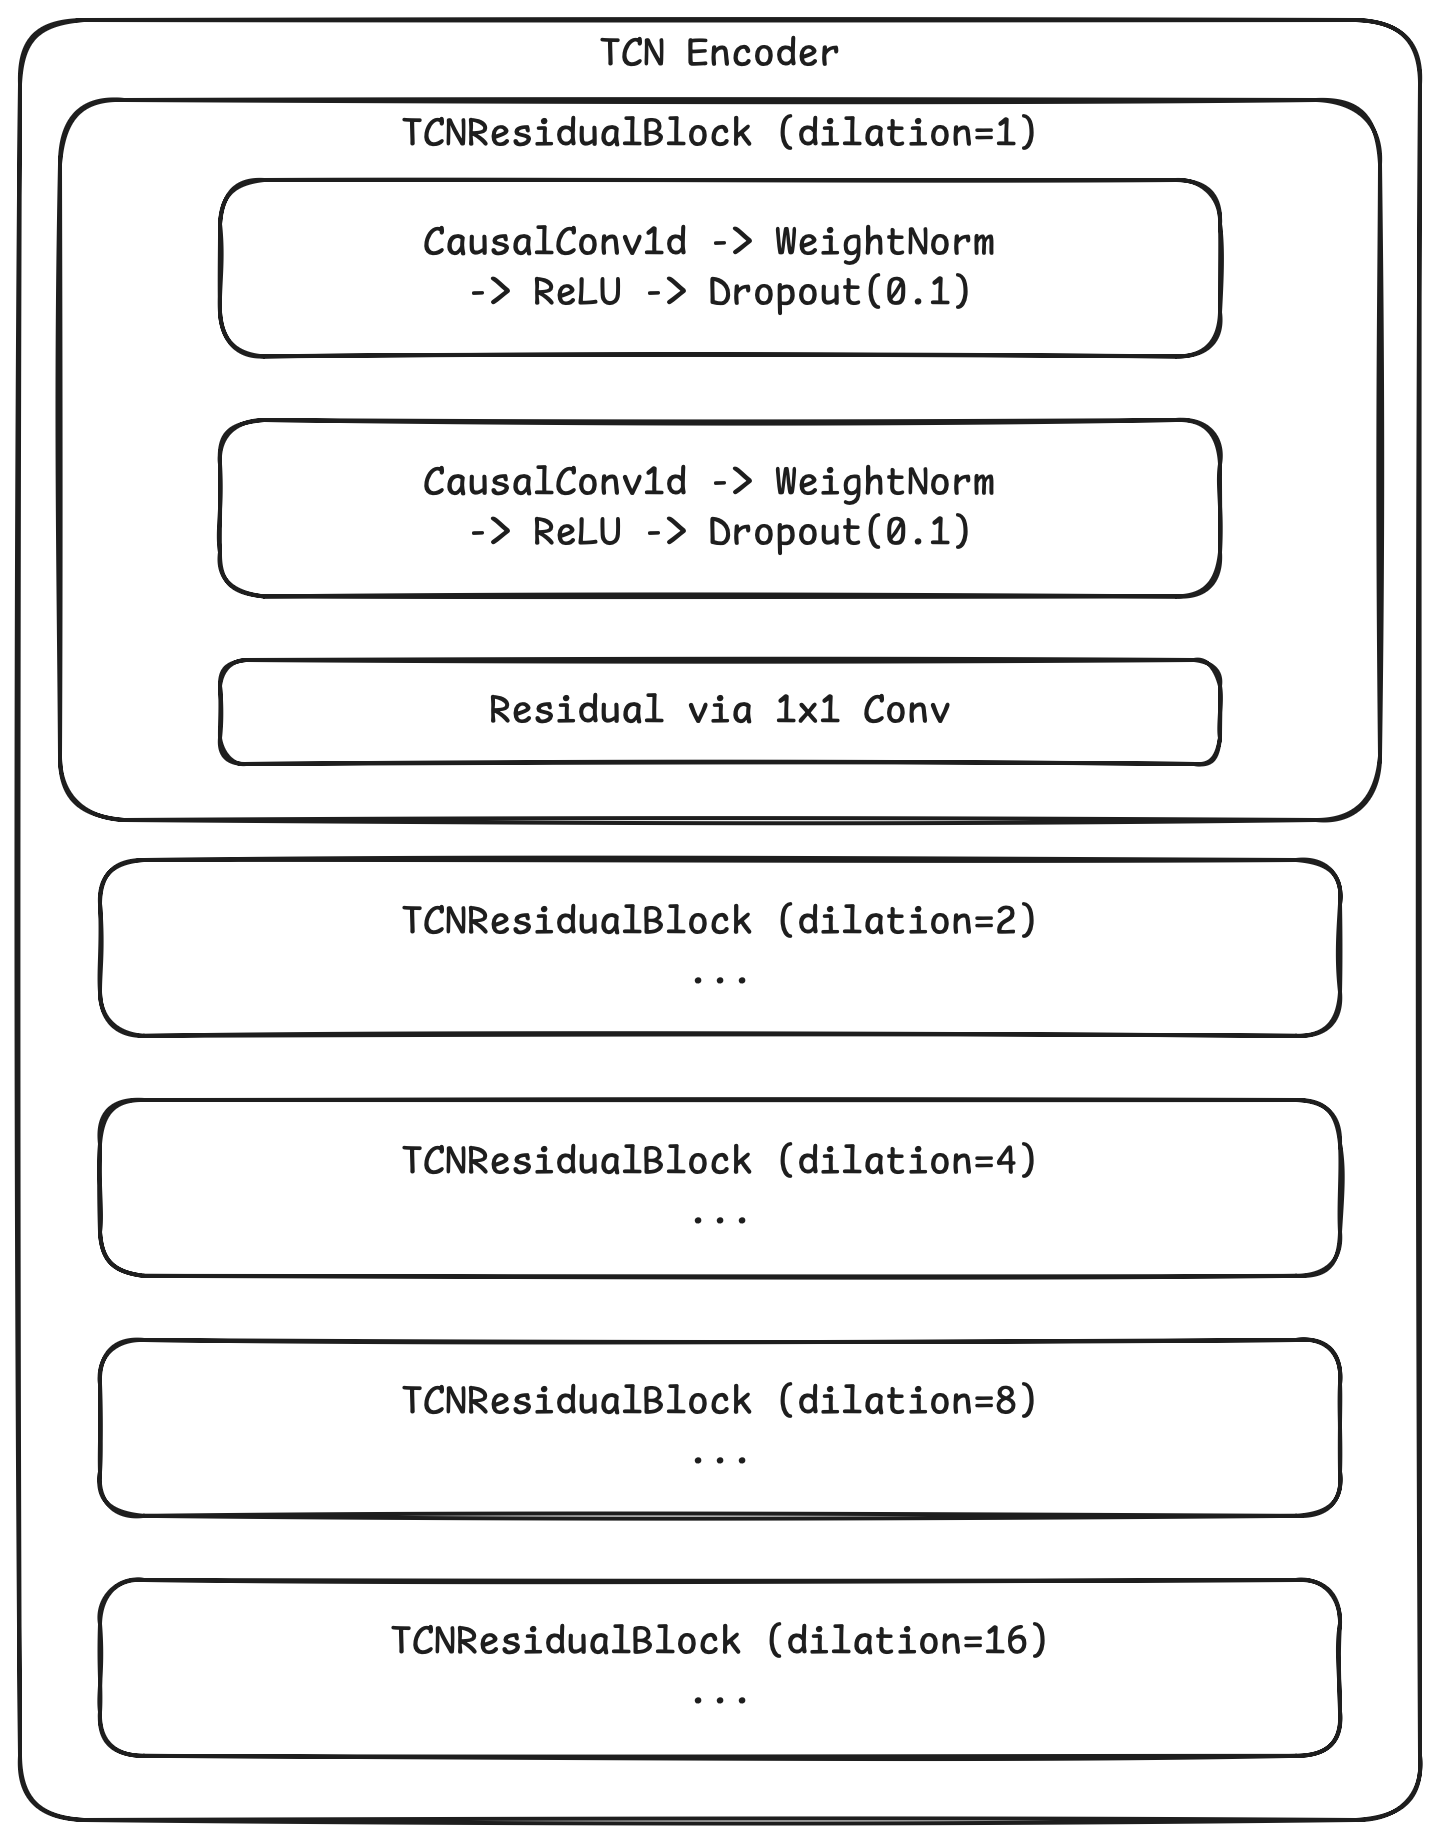
\includegraphics[width=0.48\linewidth]{figure/tcn-encoder.png}
}
\hfill
\subfloat[GRU decoder\label{fig:gru-decoder}]{%
    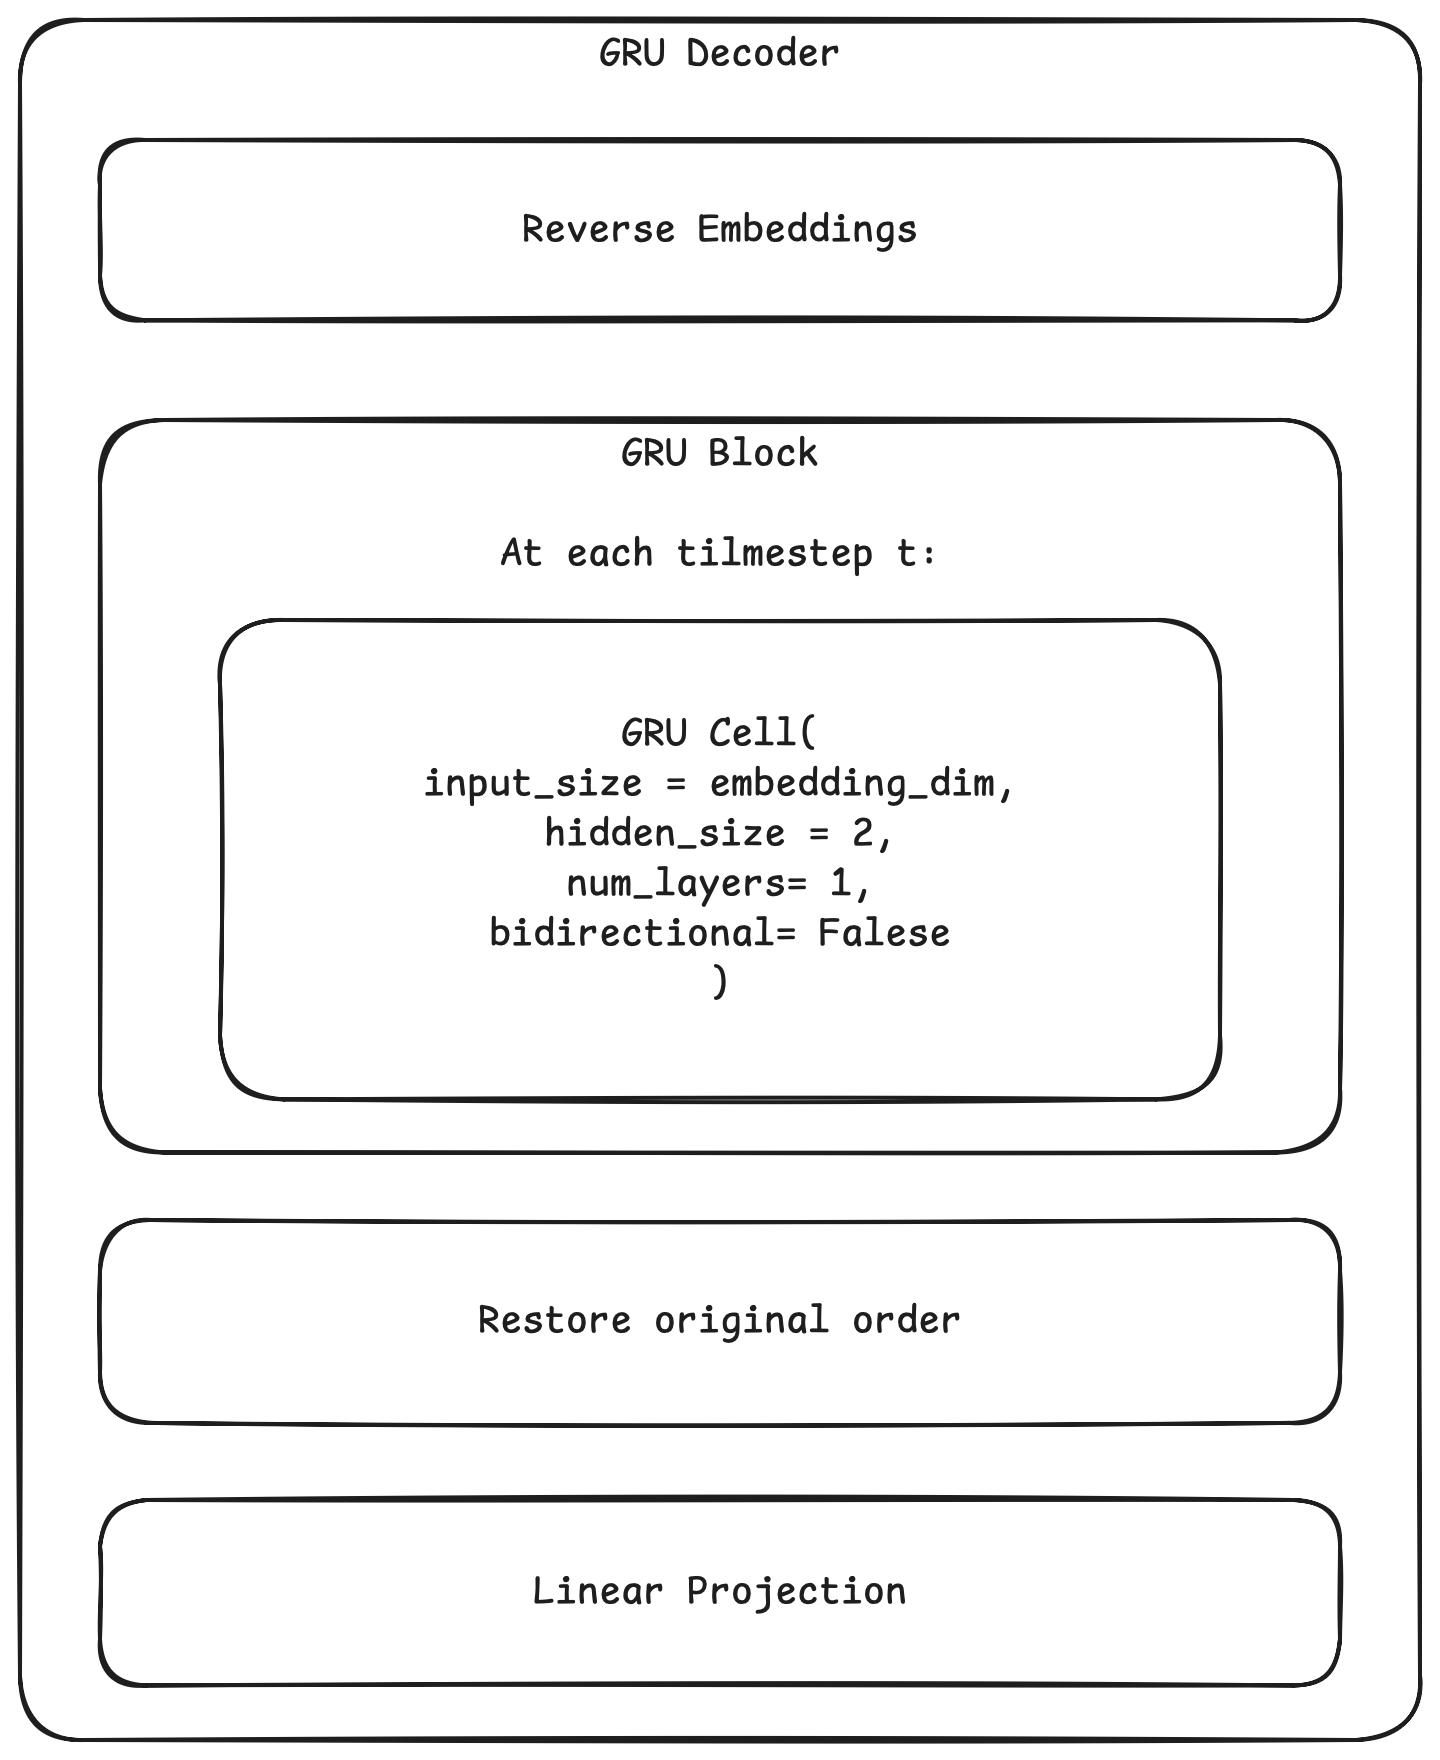
\includegraphics[width=0.48\linewidth]{figure/gru-decoder.png}
}
\caption{Detailed TCN-RNN components} % Figure text below figure
\label{fig:tcn-rnn-components}
\end{figure}

After the TCN encoder, the linear bottleneck provides the only source of geometric compression within the TCN-RNN architecture. This layer is a linear projection that reduces the input channel dimension to one. In the case of Zheng and Zhang~\cite{Zheng2023}, two input channels were used, resulting in a CR of 2:1. This means that the linear bottleneck layer of the TCN-RNN architecture produces a latent representation of the form $(\text{batch}, 1, \text{seq\_length})$.
% This is not geometric compression as we describe it above? From what I understand, geometric compression is the organization of the data in a way that allows for more effective quantization, and it importantly does not lower mutual information which a linear projection does. I'm guessing that that you are more referring to the transformation step of normal compression. (transform -> quantization -> coding). If this is the case then we should probably change the deffinition above. )

The continuous latent representation produced by the linear bottleneck serves as the input to the decoder. The decoder has two main functions. First, the embeddings are reversed for reconstruction in reverse order, meaning that the sequence is processed from end to beginning. The authors use this strategy to help the model focus on short-range temporal correlations. Second, the decoder uses a gated recurrent unit (GRU) to reconstruct the input. GRUs are a variant of RNNs that introduce reset and update gates to control the hidden state. This GRU cell expands the latent representation compressed by the bottleneck back to its original dimensionality. Afterwards, the original order is restored and a final linear projection is applied. Figure~\ref{fig:gru-decoder} shows this decoder setup in more detail.

The loss function used for the TCN-RNN baseline is identical to the loss function outlined by Zheng and Zhang~\cite{Zheng2023}. They use a simple MSE loss, but with the important caveat that they use the sum-reduced variant of MSE. The following equation shows the exact loss formula used: 

\begin{equation}
L_{\mathrm{MSE}} = \frac{1}{T} \sum_{t=1}^{T} \sum_{d=1}^{D} \left( x_t^d - \hat{x}_t^d \right)^2
\end{equation}

This function is used as the loss function for the TCN-RNN model, while the mean-reduced version of MSE is used to evaluate all the models, as described earlier in this chapter.

To validate the correctness of this implementation, a small use case from the paper is reporduced. In the paper Zheng and Zhang~\cite{Zheng2023} use the appliances energy dataset, which will be introduced at a later stage, to compress and reconstruct the two signals ``Windspeed'' and ``Appliances''. The authors present a summed MSE reconstruction error of 0.178. The implemented TCN-RNN baseline achieves a summed MSE reconstruction error of 0.133 with the same configurations, showing that it works as intended.  

\subsection{Baseline 2: EdgeCodec}

The EdgeCodec implementation leverages RVQ and a heavyweight decoder to enable a lightweight encoder architecture, which is edge-optimized~\cite{Hodo2025}. The compression mechanism of the EdgeCodec architecture is fundamentally different from the linear bottleneck employed by the TCN-RNN model. The compression achieved by EdgeCodec is a mixture of geometric compression in the encoder and compression in the information theoretic sense through quantization. The EdgeCodec encoder compresses both along the channel and the temporal axis and works as a dimensionality reduction mechanism. The quantization mechanism employed by EdgeCodec is a 4-layer hierarchical RVQ setup. The full EdgeCodec architecture is displayed in Figure~\ref{fig:edgecodec-architecture}. 

Hodo et al.~\cite{Hodo2025} provide the full code for the EdgeCodec implementation in a GitHub repository~\cite{EdgeCodec}. Therefore the EdgeCodec implementation for this thesis is largely based on this GitHub repository. An important note is that the original EdgeCodec implementation has an optional adversarial training component. For the purposes of this thesis, this is omitted, as preliminary results showed that the adversarial training component did not improve the results or was too difficult to accurately tune in the scope of this thesis. 

\begin{figure}[h]
\centering
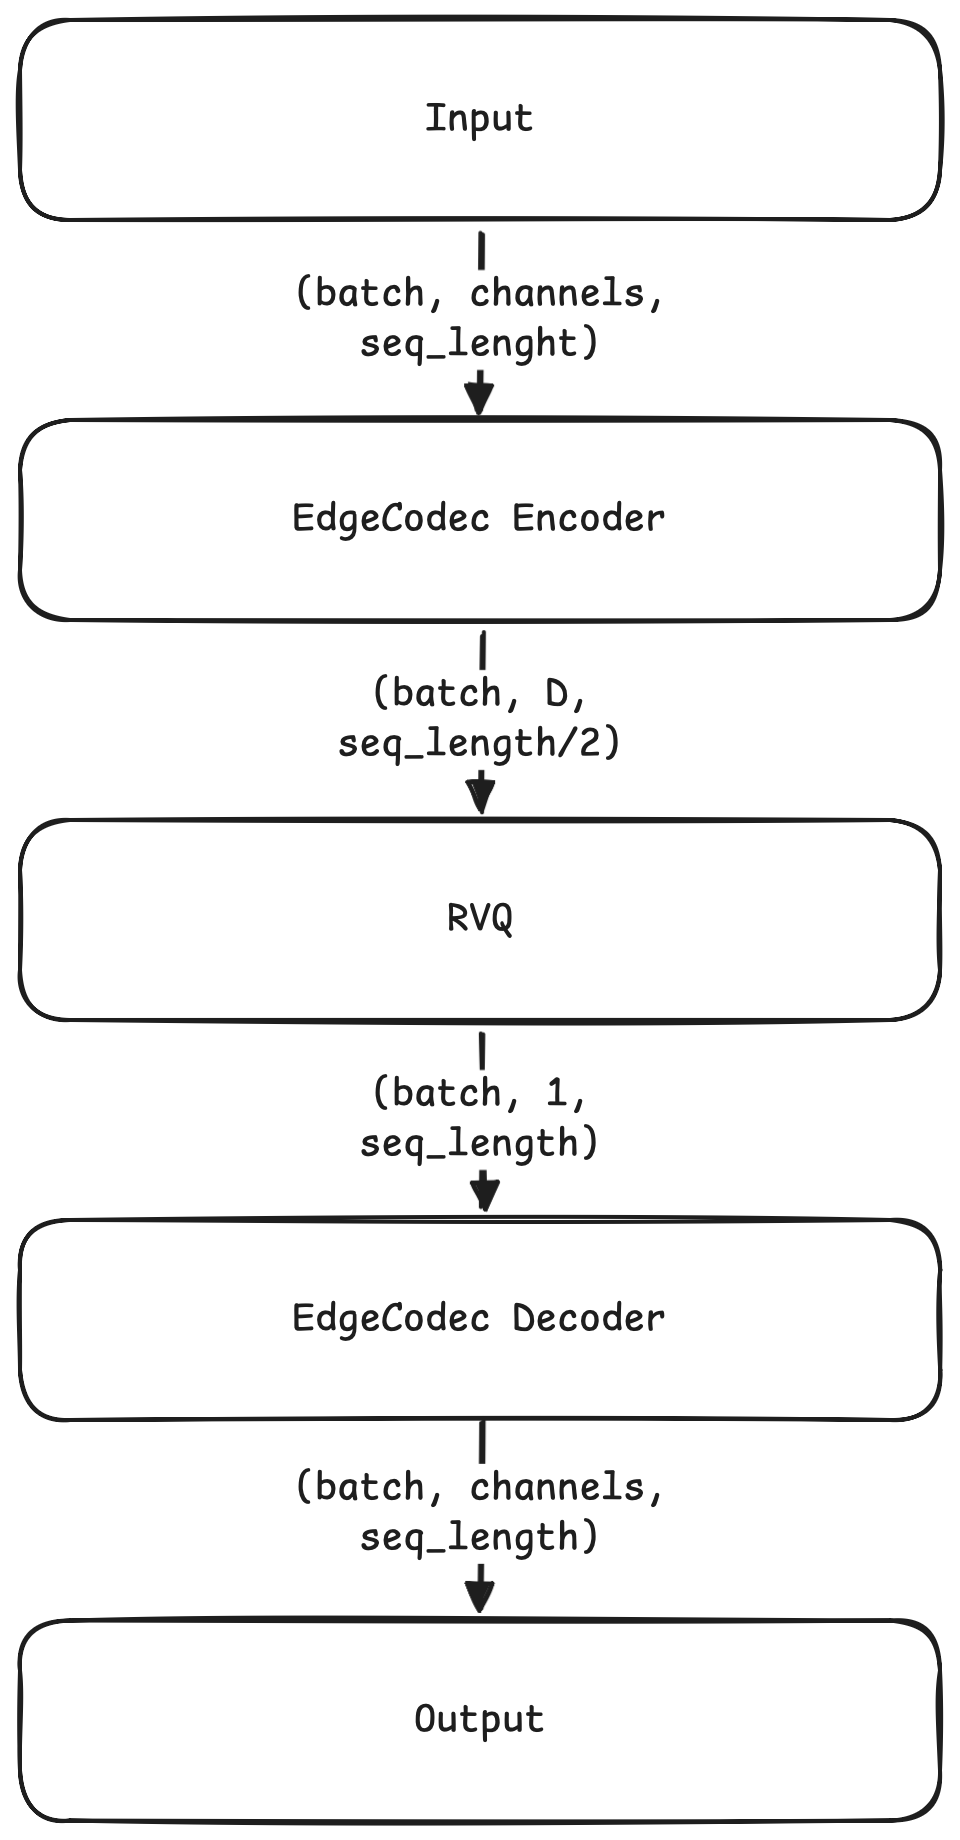
\includegraphics[width=0.40\linewidth]{figure/edgecodec.png}
\caption{EdgeCodec architecture} % Figure text below figure
\label{fig:edgecodec-architecture}
\end{figure}

The EdgeCodec encoder is intentionally lightweight. In essence, the EdgeCodec encoder architecture is fairly similar to the TCN-RNN encoder architecture. Like with the TCN-RNN encoder, the main components of the EdgeCodec encoder are residual units, which contain convolutional layers to capture local patterns. There are, however, notable differences. For one, TCN-RNN has five residual units with increasing dilation compared to the four residual units with steady dilations in the EdgeCodec encoder. Further, the EdgeCodec encoder does not use any weight normalization to optimize for computational efficiency. Another major difference between the EdgeCodec encoder and the TCN-RNN counterpart is the focus on maximizing the compression ability of the encoder. The TCN-RNN encoder employs no downsampling, neither temporal nor channel-wise. The EdgeCodec encoder actually does both. Through increasing strides, the EdgeCodec encoder is able to compress along the temporal axis, and through decreasing the input dimensionality, the EdgeCodec encoder compresses channel-wise. The CR of the EdgeCodec encoder is configurable through these two mechanisms. The detailed EdgeCodec encoder architecture with example configurations is shown in Figure~\ref{fig:edgecodec-encoder}.

\begin{figure}[h]
\centering
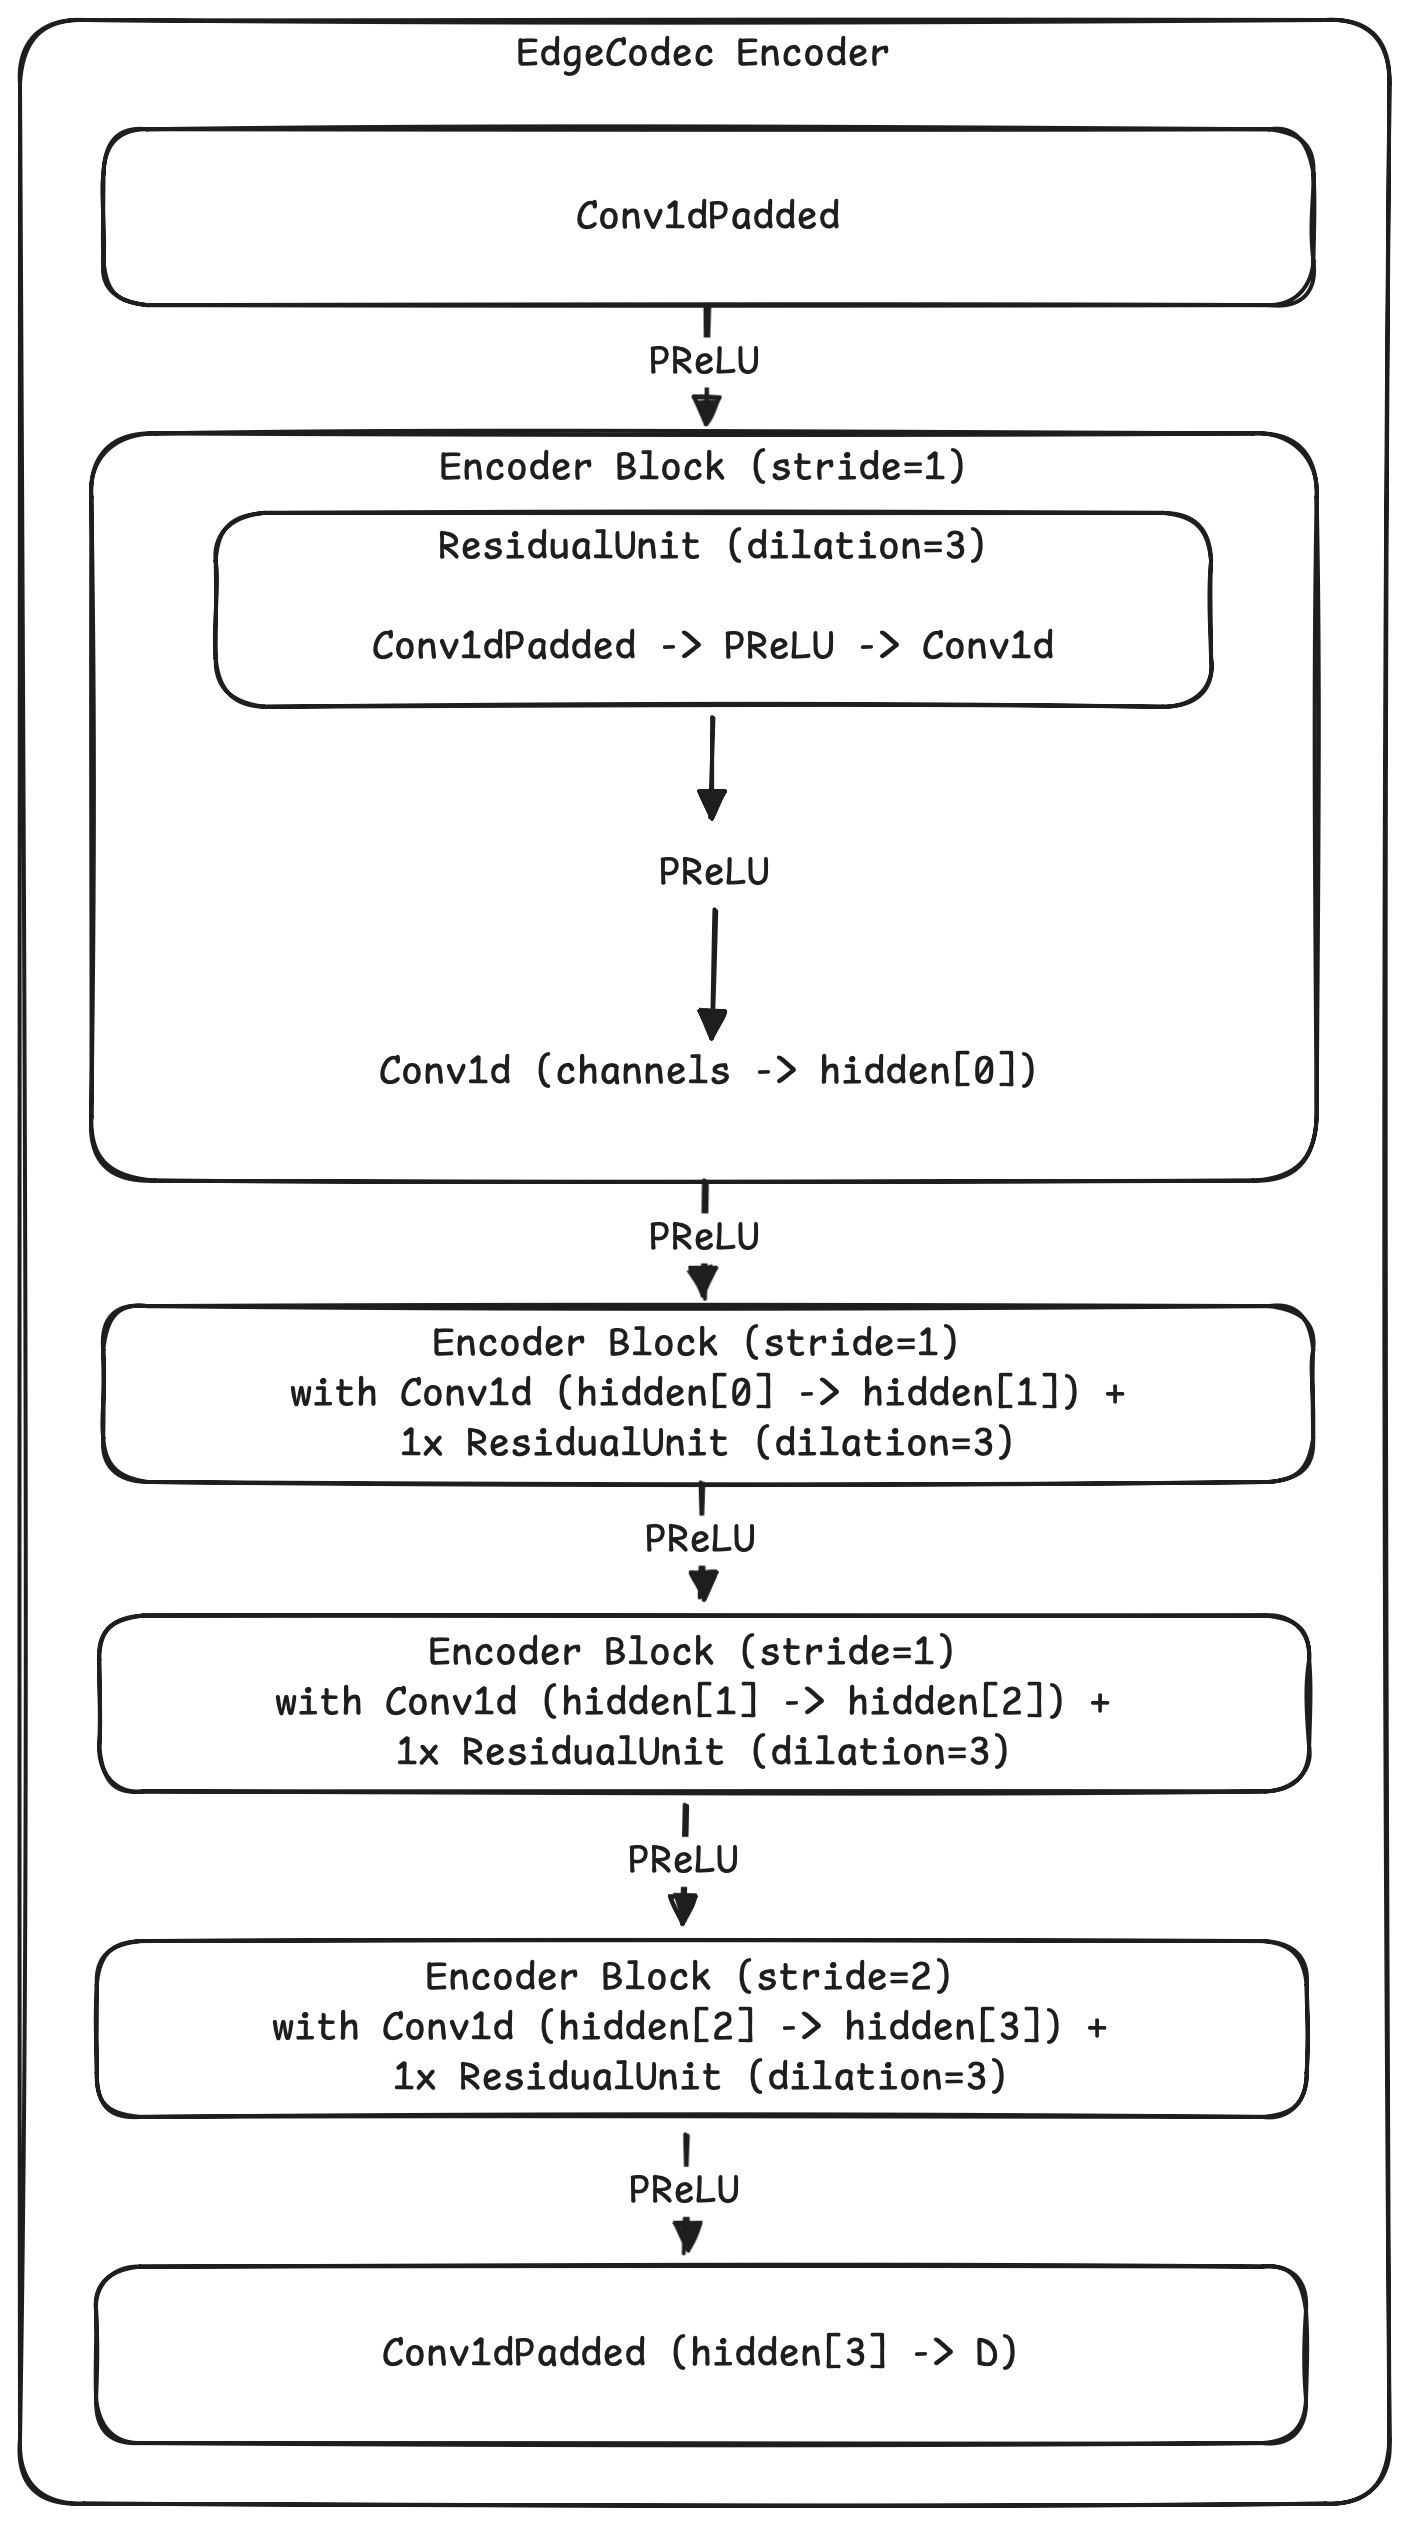
\includegraphics[width=0.40\linewidth]{figure/edgecodec-encoder.png}
\caption{EdgeCodec encoder} % Figure text below figure
\label{fig:edgecodec-encoder}
\end{figure}

Because the EdgeCodec encoder is purposefully kept lightweight, the authors compensate through a more complex and heavyweight decoder. The EdgeCodec decoder mainly implements this through channel-wise linear layers that process each channel independently. Two of these channel-wise linear layers are implemented in the EdgeCodec decoder architecture, one at the beginning and one in the middle after the first two decoder blocks. The decoder blocks are also more heavyweight compared to the encoder blocks used in the EdgeCodec encoder. Instead of only one residual unit, the decoder block implements three residual units with increasing dilation to enhance its capabilities in modeling long-range temporal patterns. The downsampling pattern along the temporal and channel-wise axis implemented in the EdgeCodec encoder is mirrored by the EdgeCodec decoder to restore the original input shape. A detailed architectural overview of the EdgeCodec decoder is presented in Figure~\ref{fig:edgecodec-decoder}.

\begin{figure}[h]
\centering
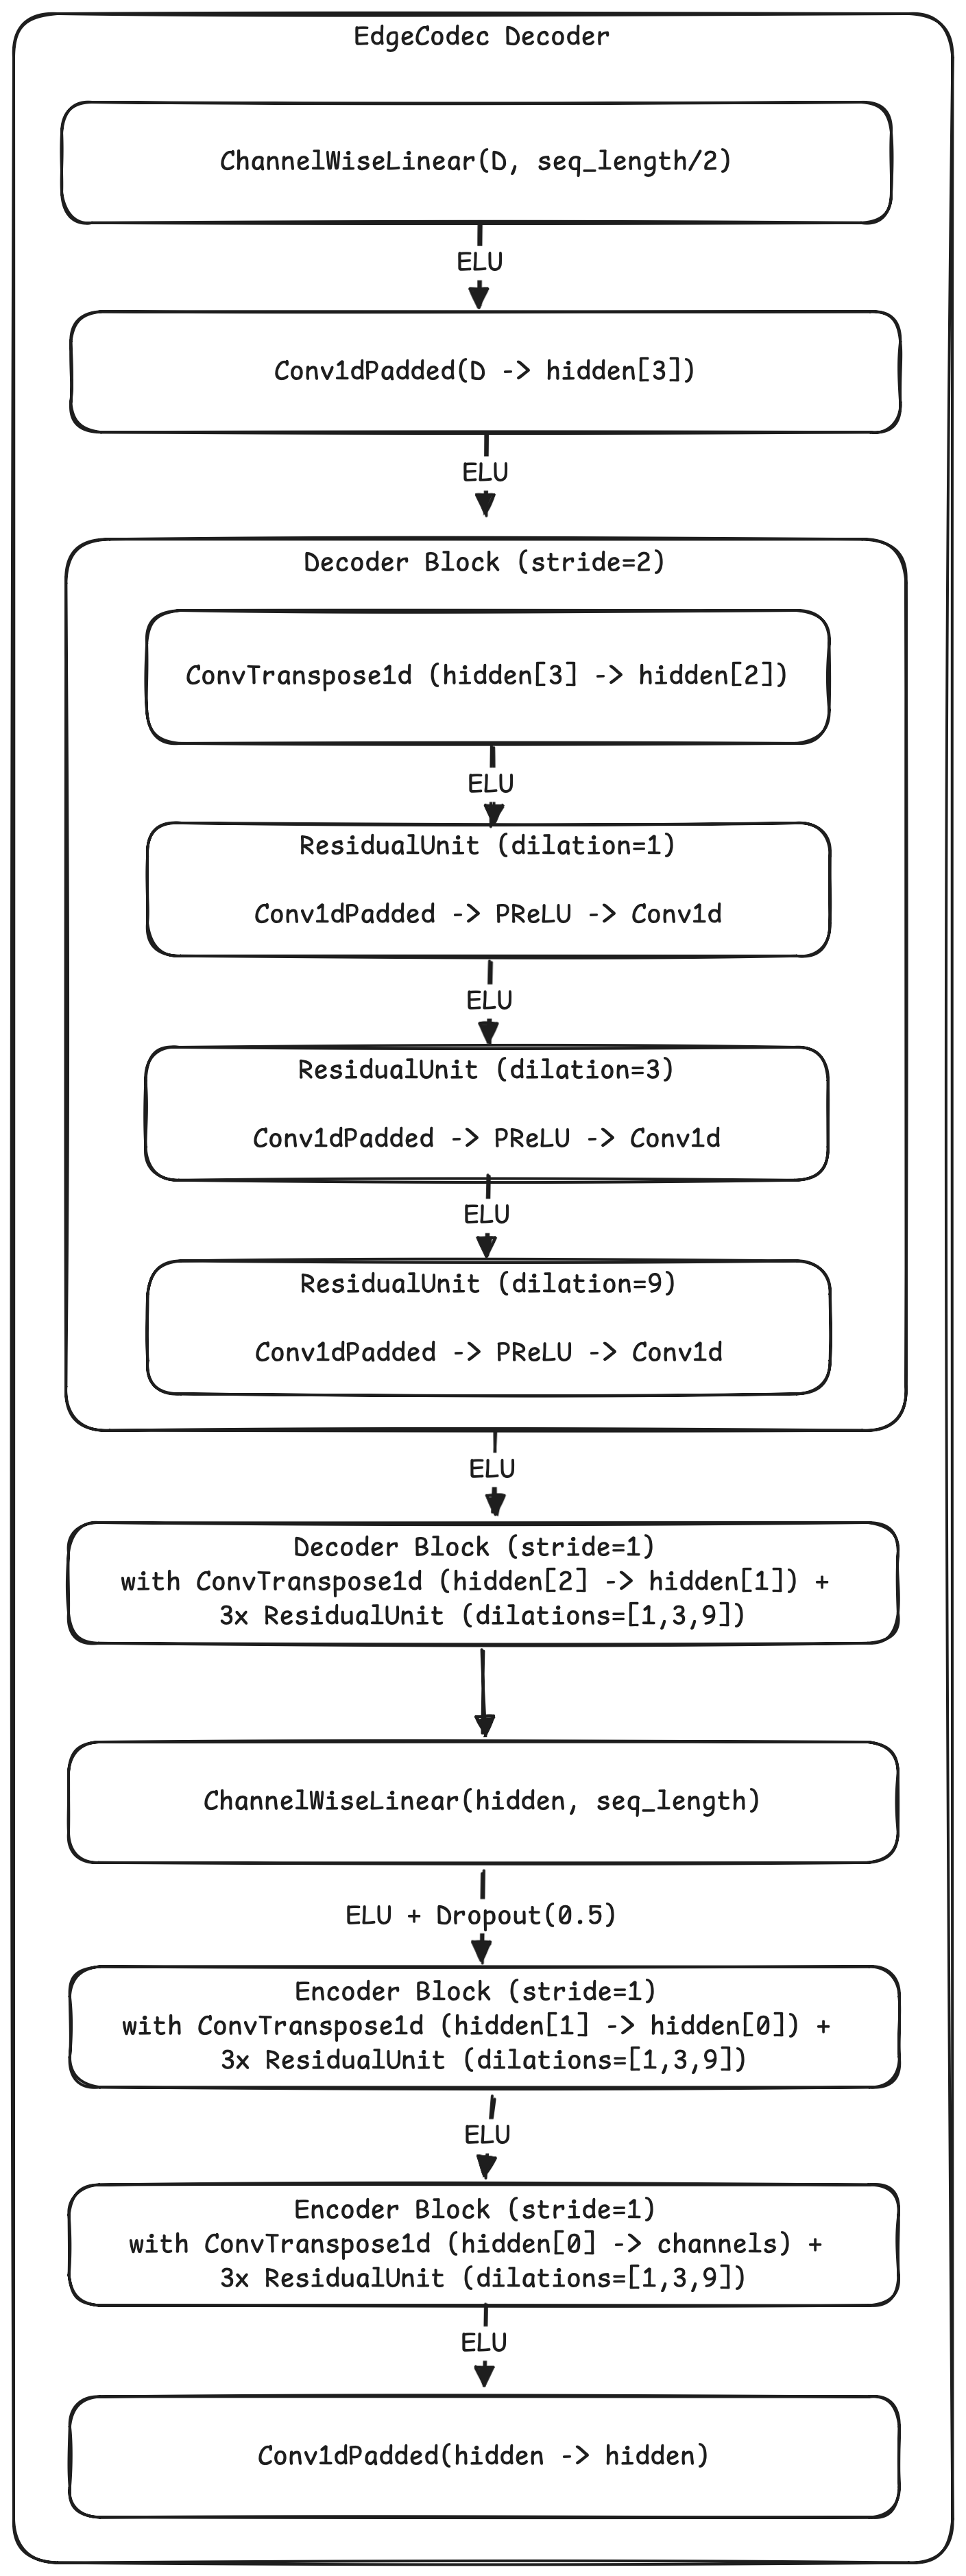
\includegraphics[width=0.30\linewidth]{figure/edgecodec-decoder.png}
\caption{EdgeCodec decoder} % Figure text below figure
\label{fig:edgecodec-decoder}
\end{figure}

Although differences in the encoder and decoder structure between the TCN-RNN and the EdgeCodec architecture are substantial, the most substantial difference between the TCN-RNN model and the EdgeCodec model is the use of a quantization mechanism to produce discrete latents. EdgeCodec utilizes a 4-level hierarchical RVQ setup to learn the codebooks. The implementation of RVQ is standardized in most modern neural compression methods through the \textit{vector-quantize-pytorch} library by Phil Wang~\cite{LucidrainsVQPT}. Hodo et al.~\cite{Hodo2025} initialize the RVQ method using embedding dimensions equal to the sequence length divided by the temporal compression of the encoder. For example, if the input has a sequence length of 128, and the encoder compresses this with a temporal CR of 2:1, the embedding dimensions for the RVQ method are 64. This enables the RVQ mechanism to assign one codebook per sequence for each channel. The non-differentiability and the resulting challenging end-to-end training of quantization methods has already been discussed above. RVQ handles this by employing exponential moving average (EMA) training, which enables more stable codebook updates compared to gradient-based training.

The loss function used to train EdgeCodec combines reconstruction error, quantization loss, and optional adversarial loss:

\begin{equation}
L(x, \hat{x}, z, \tilde{z}, y, g) = \alpha \cdot L_\mathrm{MSE}(x, \hat{x}) + (1 - \alpha) \cdot L_{l1\mathrm{-smooth}}(x, \hat{x}) + \eta \cdot L_\mathrm{RVQ}(z, \tilde{z}) + \gamma \cdot L_\mathrm{adv}(y, g)
\end{equation}

where $x$ is the input, $\hat{x}$ is the reconstructed output, $z$ and $\tilde{z}$ are the original and quantized latents, $y$ and $g$ represent the discriminator and generator outputs, and $\alpha, \eta, \gamma$ are weighting coefficients. As described before, for the purposes of this thesis, the adversarial training loss is omitted.

Because the presented implementation of the EdgeCodec baseline is heavily based on the provided code by the authors and largely reproduced one to one, an experiment to validate the correctness of this reproduction of the EdgeCodec model is omitted. 